\documentclass{article}
\usepackage[utf8]{inputenc}
\usepackage{amsmath}
\usepackage{amssymb}
\usepackage{graphicx}
\usepackage{epstopdf}
\usepackage{inputenc}
\usepackage[version=4]{mhchem}
\usepackage{commath}
\usepackage{graphicx}

\documentclass{article}
\usepackage{xcolor}
\usepackage{listings}

\definecolor{mGreen}{rgb}{0,0.6,0}
\definecolor{mGray}{rgb}{0.5,0.5,0.5}
\definecolor{mPurple}{rgb}{0.58,0,0.82}
\definecolor{backgroundColour}{rgb}{0.95,0.95,0.92}

\lstdefinestyle{CStyle}{
    backgroundcolor=\color{backgroundColour},   
    commentstyle=\color{mGreen},
    keywordstyle=\color{magenta},
    numberstyle=\tiny\color{mGray},
    stringstyle=\color{mPurple},
    basicstyle=\footnotesize,
    breakatwhitespace=false,         
    breaklines=true,                 
    captionpos=b,                    
    keepspaces=true,                 
    numbers=left,                    
    numbersep=5pt,                  
    showspaces=false,                
    showstringspaces=false,
    showtabs=false,                  
    tabsize=2,
    language=C
}

\begin{document}
\title{Combined Temperature and Pressure Sensor with Display Based on the MSP 430 Microprocessor}
\author{Muchen He}
\date{April 5, 2022}
\maketitle

\section{Abstract}
Using the microprocessor, we have designed, constructed and tested a Combined Temperature and Pressure Sensor that can be applied in many household scenarios as well as industrial scenarios, such as monitoring the room temperature and pressure, regulating the temperature of a wine cellar, or monitoring the pressure and temperature of a pressured device. It has the advantage of being easy to set up with just a few  components, a power source, and a computer. It is also very flexible and can be integrated into a system due to the flexibility of the microprocessor. With the ADC communication function and interrupt function of the MSP430G2553 Microprocessor, we are able to obtain data from the TMP 36 Temperature Sensor and the abpdant005pgaa5 Pressure Sensor, then display the data using a seven-segment display with high precision. 

The combined sensor works within a large range of pressure and temperature: 0°C  to 99 °C, and up to $34\%$ difference from atmospheric pressure. It is also very precise, with a $\pm$ 0.1 \textdegree C error for the temperature reading, and 1.5 $\%$ error to the pressure reading. The project also comes with 3 different code packages to use in different conditions:

\begin{enumerate}
    \item Continuous:  The sensor continuously displays pressure or temperature, alternating in 5 seconds cycles.  The display updates every 0.1 s
    \item Alternating:  Each time a button is pressed, the sensor alternates between pressure and temperature and the display updates once. 
    \item Semi-Continuous: The sensor alternates between displaying temperature and pressure once with each press, then with each press of the button, does five second continuous display cycle, and going back to alternating. 
\end{enumerate}
If needed, the template code can be used to add and modify the components easily.

\section{Introduction}
For this project, we have designed coded and constructed a combined pressure and temperature sensor integrated with a seven segment display, based on the MSP430G2553 microprocessor. The project is mainly based around 2 of the main abilities of the MSP430: the ADC conversion and the interrupt. In this report, I will go through the apparatus, setting up the sensor, reading the display, the code, measurement precision, results and testing, discussion and improvements, and the conclusion of the project.

\section{Apparatus} 
For the construction of the circuit, we used several components, including:
\begin{enumerate}
  \item Protoboard with Ground, 3.3V and 5.0V power supply. 
  \item Required USB and other types of plugs and wires. 
  \item TMP 36 Temperature Sensor
  \item abpdant005pgaa5 Pressure Sensor
  \item MSP430G2553 Microprocessor
  \item Seven Segment Display (UBC Provided, Based o nDM9368 7-Segment Decoder with 74HC/H CT139 Dual 2-to-4 line decoder) 
\end{enumerate}

The construction of the project is, to put simply, connecting the wires. Please refer to the circuit diagram for the construction (Figure 1).  Notice the only extra available pins are P1.5, P1.7 and P2.3 since P1.3 is the button, and P1.0 and 1.6 are used for the LED lights. 

\begin{figure}[h]
    \centering
    \includegraphics[width=6cm]{Circuit Diagram.jpg}
    \caption{The circuit diagram for the combined sensor}
\end{figure} 

The end product of the circuit is attached below as well (see figure 2 and 3). 

\begin{figure}[h]
    \centering
    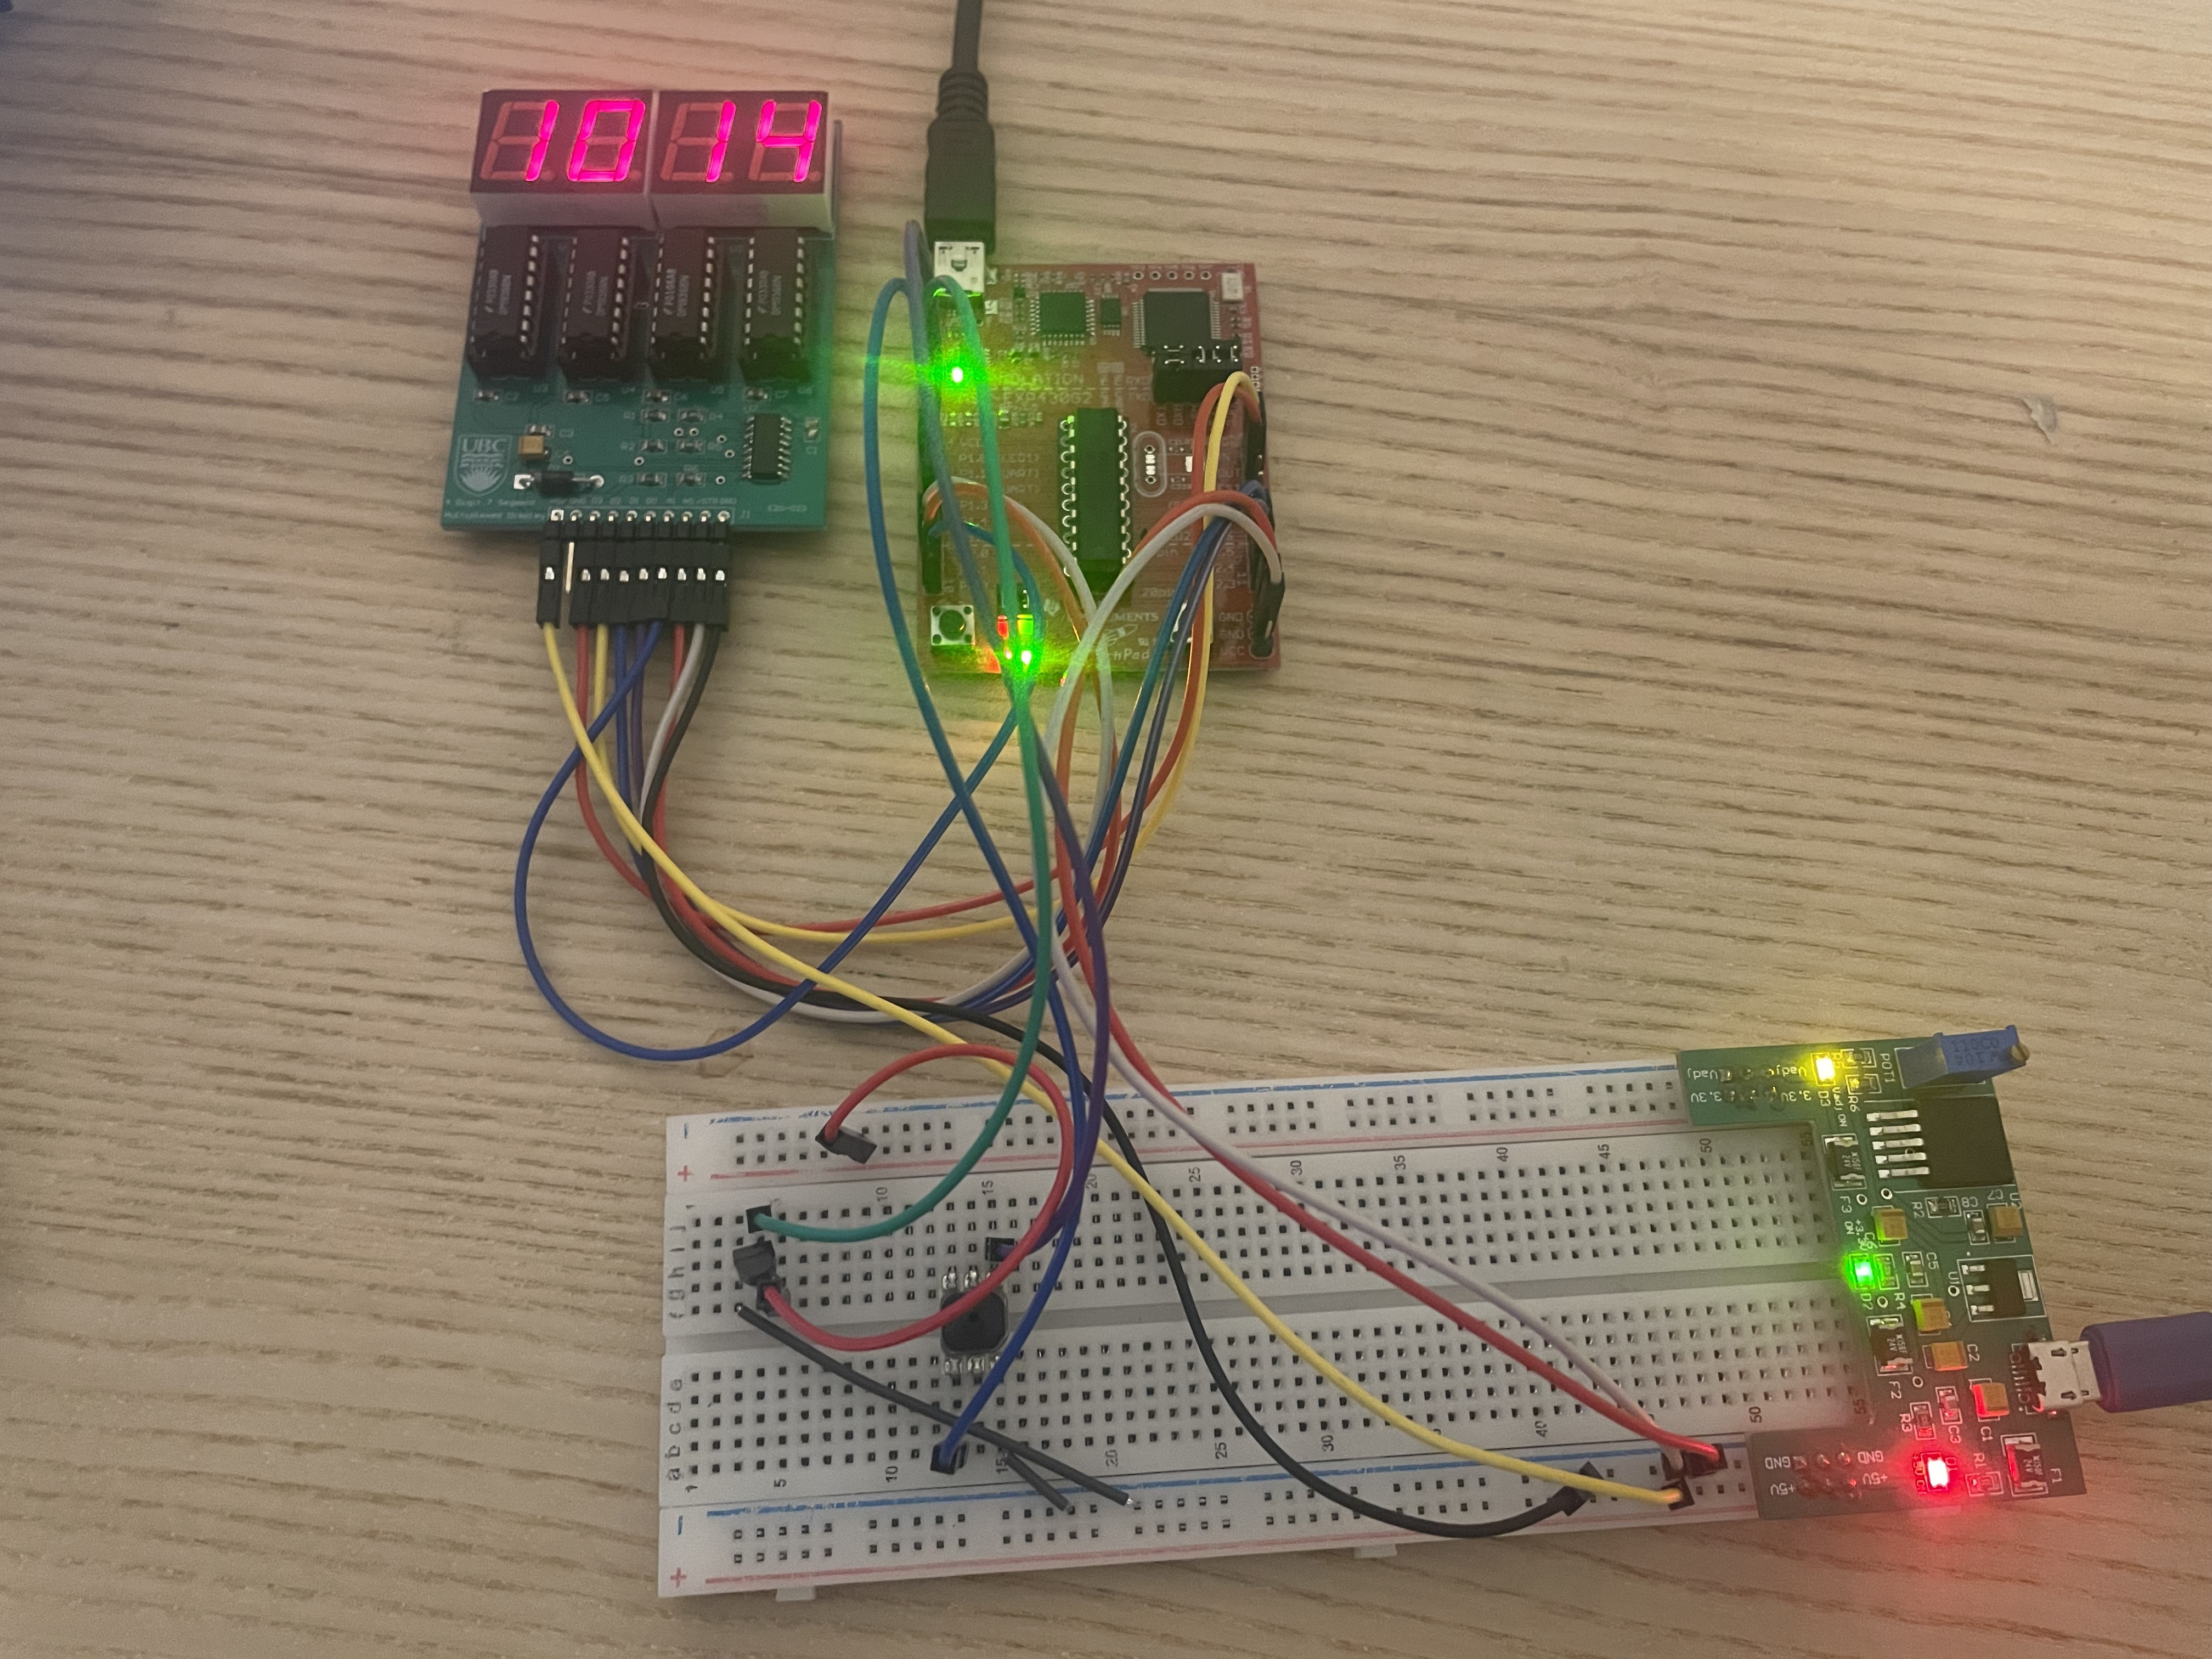
\includegraphics[width=6cm]{Displaying Pressure.png}
    \caption{The sensor setup displaying pressure}
\end{figure} 

\begin{figure}[h]
    \centering
    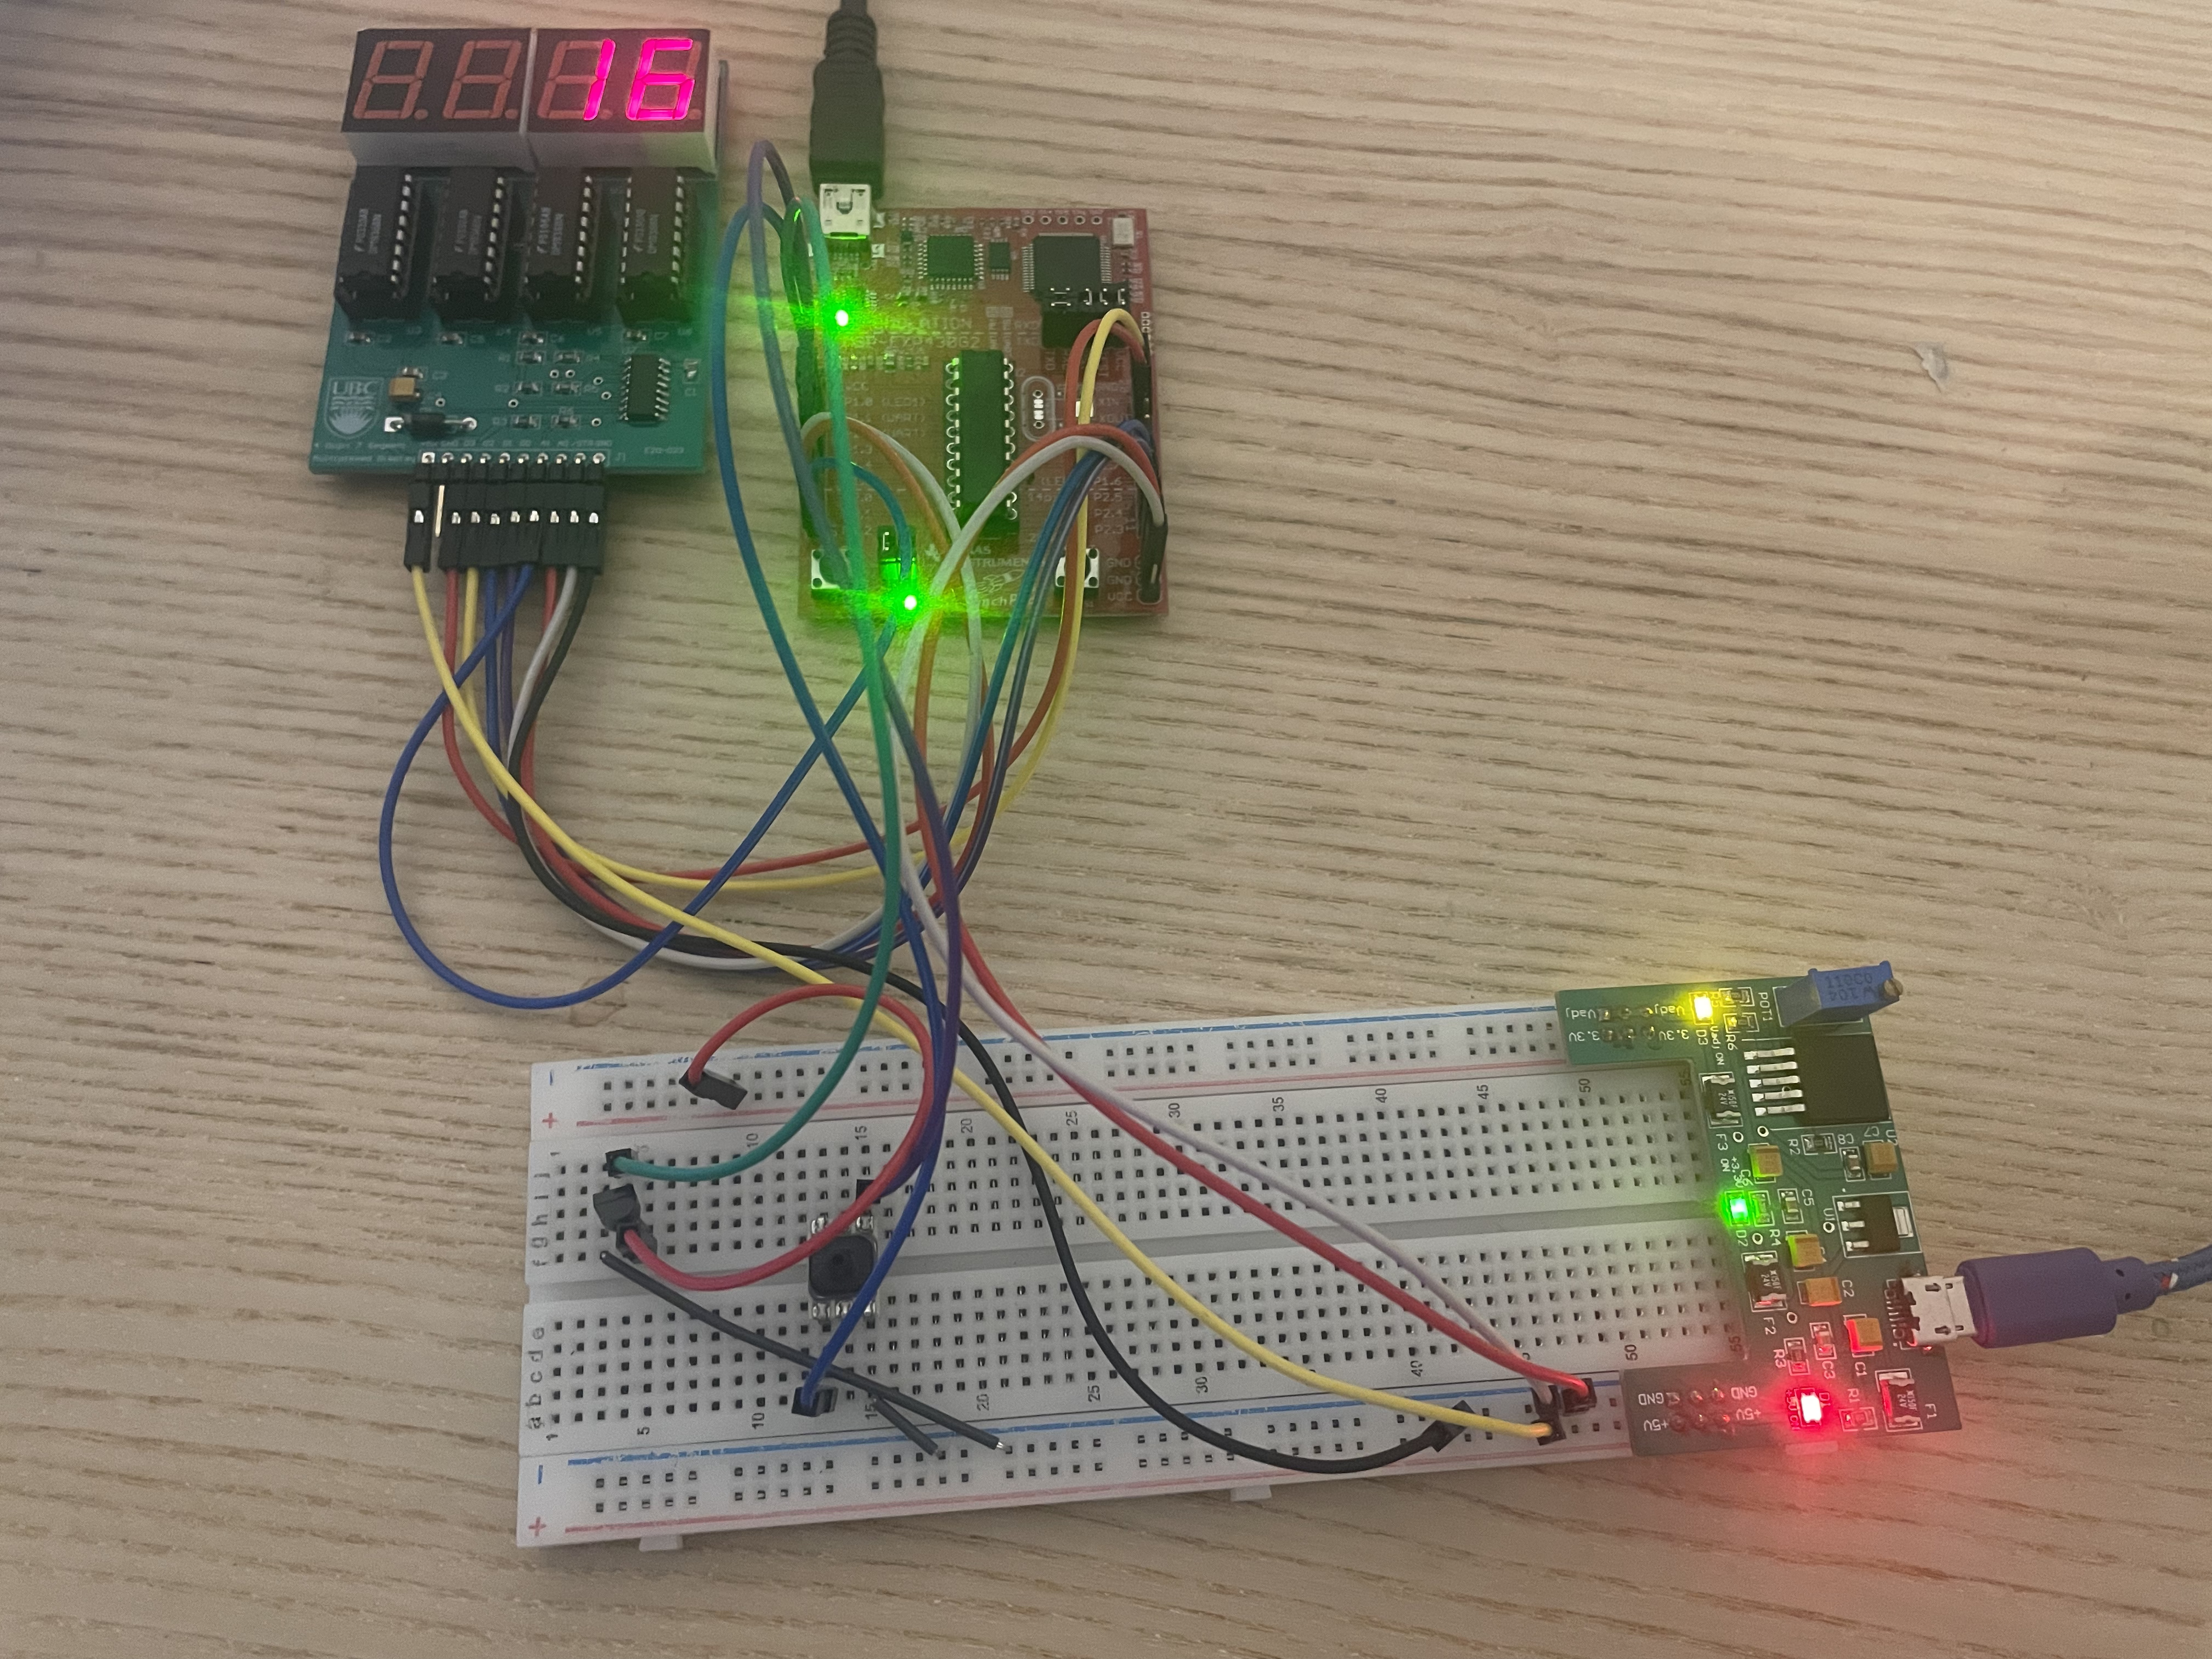
\includegraphics[width=6cm]{Diplaying Temperature.png}
    \caption{This the sensor setup displaying temperature}
\end{figure} 

\section{Setting Up the Sensor}
The sensor is easy to setup. First obtain the required parts and construct the sensor. With a computer, download Code Composer 11.1.0, and the required code packages. Import the package into the code composer, then connect the Microprocessor to the computer, and the protoboard to a power source. First press 'build', then press 'debug'. After the computer has successfully loaded the program onto the MSP 430, press Run. Then the MSP 430 can be connected to an external power source and will run as desired. 

\section{Reading the Display}
Reading the display is simple. When a one digit or two digit number is displayed, the display is displaying the temperature in a range of 0 - 99 degrees. Since pressure meter only works with 34\% range of atmospheric, or measures a minimum of around 650 millibars. The value displayed is in degrees. When a three or four digit number is displayed, we are displaying the pressure in millibars. 

\section{Code} 
We will not have the code here. The code will be attached separately from the report. For the code, please refer to my github page https://github.com/MuchenHe [1]. The code was completed in C using code composer, then loaded onto the MSP430 via a computer connection. 

For the combined sensor, we have completed 3 different code packages, to serve three different functions. 

The first package is the most basic function. It will allow the sensor to alternate through sensing and displaying of temperature and pressure. It starts with the interrupt ability of the MSP 430. The microprocessor comes with a button that can be applied to this function on P1.3. With the press of this button, we can start the sensor, and alternate between the display of Temperature and humidity. This is achieved by running the command 

\begin{lstlisting}[style=CStyle]
P1OUT = BIT3 + BIT0;
P1REN = 0b00001000; //enable pull up/down resistor on P1.3
P1IE = 0b00001000; //Enable input at P1.3 as an interrupt
 _BIS_SR(LPM4_bits + GIE); //Turn on interrupt
\end{lstlisting}
with in the main() function. Here, we set P1.3 to high and enable pull down resistor on P1.3. Then we enable the following interrupt function: 
\begin{lstlisting}[style=CStyle]
void __attribute__((interrupt(PORT1_VECTOR))) PORT1_ISR(void) { 
\\Function Body
}
\end{lstlisting}
We have an if/else if statement inside the interrupt function body, which allows us to cycle through temperature or pressure with each press (i.e. running the function again). This function may look something like this: 
\begin{lstlisting}[style=CStyle]
if (acc == 0) {
    \\Measure and display the temperature
    acc = 1; 
}

else if (acc == 1) {
    \\ Measure and display the pressure
    acc = 0; 
}
\end{lstlisting}

For the data collection and transmission from the temperature sensor and the pressure sensor to the microprocessor, we use the ADC transmission function, since both of these sensors are analog. The ADC transmission measures the voltage as a number which is the variable ADC10MEM. We set up the ADC transmission function using the following snippet of code:
\begin{lstlisting}[style=CStyle]
 // This configures ADC, see lab Part 5
        ADC10CTL0 = ADC10SHT_2 + ADC10ON; // ADC10ON
        ADC10CTL1 = INCH_2; //We read in on P1.2
        ADC10AE0 |= 2; // PA.1 ADC option select

        ADC10CTL0 |= ENC + ADC10SC; // Sampling and conversion start
        while (ADC10CTL1 & ADC10BUSY); // ADC10BUSY?
\end{lstlisting}

where 'ADC10CTL1 = INCH\_2;' tells us which port we are reading in from. From this code, we will obtain a value stored in ADC1OMEM. Then, ADC10MEM is divided by 1023 would give us the voltage at the specific port out of 3.3V. From the data sheets and other sources, we have calculated the conversion ratio for temperature[2] (in degrees) to be
\begin{align}
    \frac{3.2258ADC10MEM - 500}{10} 
\end{align}
and the conversion to pressure (in millibars) [3] to be 
\begin{align}
    68.9(14.696 + \frac{25ADC10MEM}{4092})
\end{align}
And each of these are converted into an array of 4 integers, and using the seven segment display library from Alex[4] which was edited to work with Pin 2, we are able to display these values. I will attach an example of how this works:
\begin{lstlisting}[style=CStyle]

        unsigned char pressure_arr[4];
        
        pressure_arr[0] = (unsigned char)(pressure_millibar / 1000);
        pressure_arr[1] = (unsigned char)((pressure_millibar % 1000) / 100);
        pressure_arr[2] = (unsigned char)((pressure_millibar % 100) / 10);
        pressure_arr[3] = (unsigned char)(pressure_millibar % 10);

        set_strobe(1);

        set_display_from_nums(pressure_arr);
        
\end{lstlisting}
Other parts that needed to be mentioned about this code is using P2.6 and P2.7. We notice that there are no P2.6 and P2.7 on the microprocessor. But we are able to use the pins XIN and XOUT as these to pins with the command 'P2SEL \&= ~0xC0;'. 

The second package is a slight variation of the first to serve a few functions. We basically use the same construction as the previous function, but we add additional ability to display the temperature data or pressure data continuously (updates every 0.1 seconds). For this code package, our display first displays the temperature once, then the pressure, then the temperature which updates continuously for 5 second, and then the pressure continuously for 5 seconds. The cycles are achieved with the following structure embedded into the if statements: 
\begin{lstlisting}[style=CStyle]
for (acc_continuous = 0; acc_continuous < 50; acc_continuous++) {
                \\Measure and display the data
                _delay_cycles(100000);
                }
\end{lstlisting}

And the last package is the most simple one. It just display the temperature then pressure in 5 second cycles forever. Here, we use a while loop to keep it running forever. This will look something like: 
\begin{lstlisting}[style=CStyle]
while (1) {
\\ display and measurement alternating between temperature and pressure
}
\end{lstlisting}
Please refer to the github page for more infomation [1].  

Each of these package can be used in a different scenario; whether continuous monitoring is needed, or if one time updates are needed, there is a package to do the job. 

\section{Precision} 
Another important part to discuss about a sensor is its precision. This sensor is more precise than needed in most household scenarios. The temperature is has an accuracy of $\pm$ 0.1 \textdegree C error, much less that that what our display displays (we display to integer value); Thus we can conclude that the temperature displayed is accurate to $\pm$ 0.5  \textdegree C. The pressure has an error of 1.5$\%$ according to the data sheet. Notice this 1.5$\%$ error is for the relative pressure of the measured pressure and STP, so the at close to atmospheric, the error is extremely small. 

\section{Results and Testing}
Testing is very important to ensure that each component is working correctly. We first start by testing the code that switches between measuring temperature and pressure. We assigned different lighting arrangements (green light/red light), on the MSP 430, and we have confirmed that this section of the code indeed works.

The we tested the display code by manually feeding in different display values and this confirmed the display to work. Notice within the range of 0-99 degrees, we will never get an 'illegal' number that we cannot display, and the pressure will never be an 'illegal' number, since the pressure sensor only works up to $34\%$ difference from atmospheric pressure. 

Lastly we test the whole code to see if it's working correctly. We run the code, and compare the displayed pressure and temperature data to the ambient temperature and pressure. Our pressure agrees with air pressure published on weather report that day, and our temperature agrees with the indoor temperature of the lab. Furthermore, we have demonstrated that with a syringe, that the pressure sensor reading changes accordingly as we compress the air (see figure 4). Similarly, our temperature reading changes as expected as we use a human heat source to heat up the sensor (see figure 5). Thus we believe that our sensor is working accordingly. 

\begin{figure}[h]
    \centering
    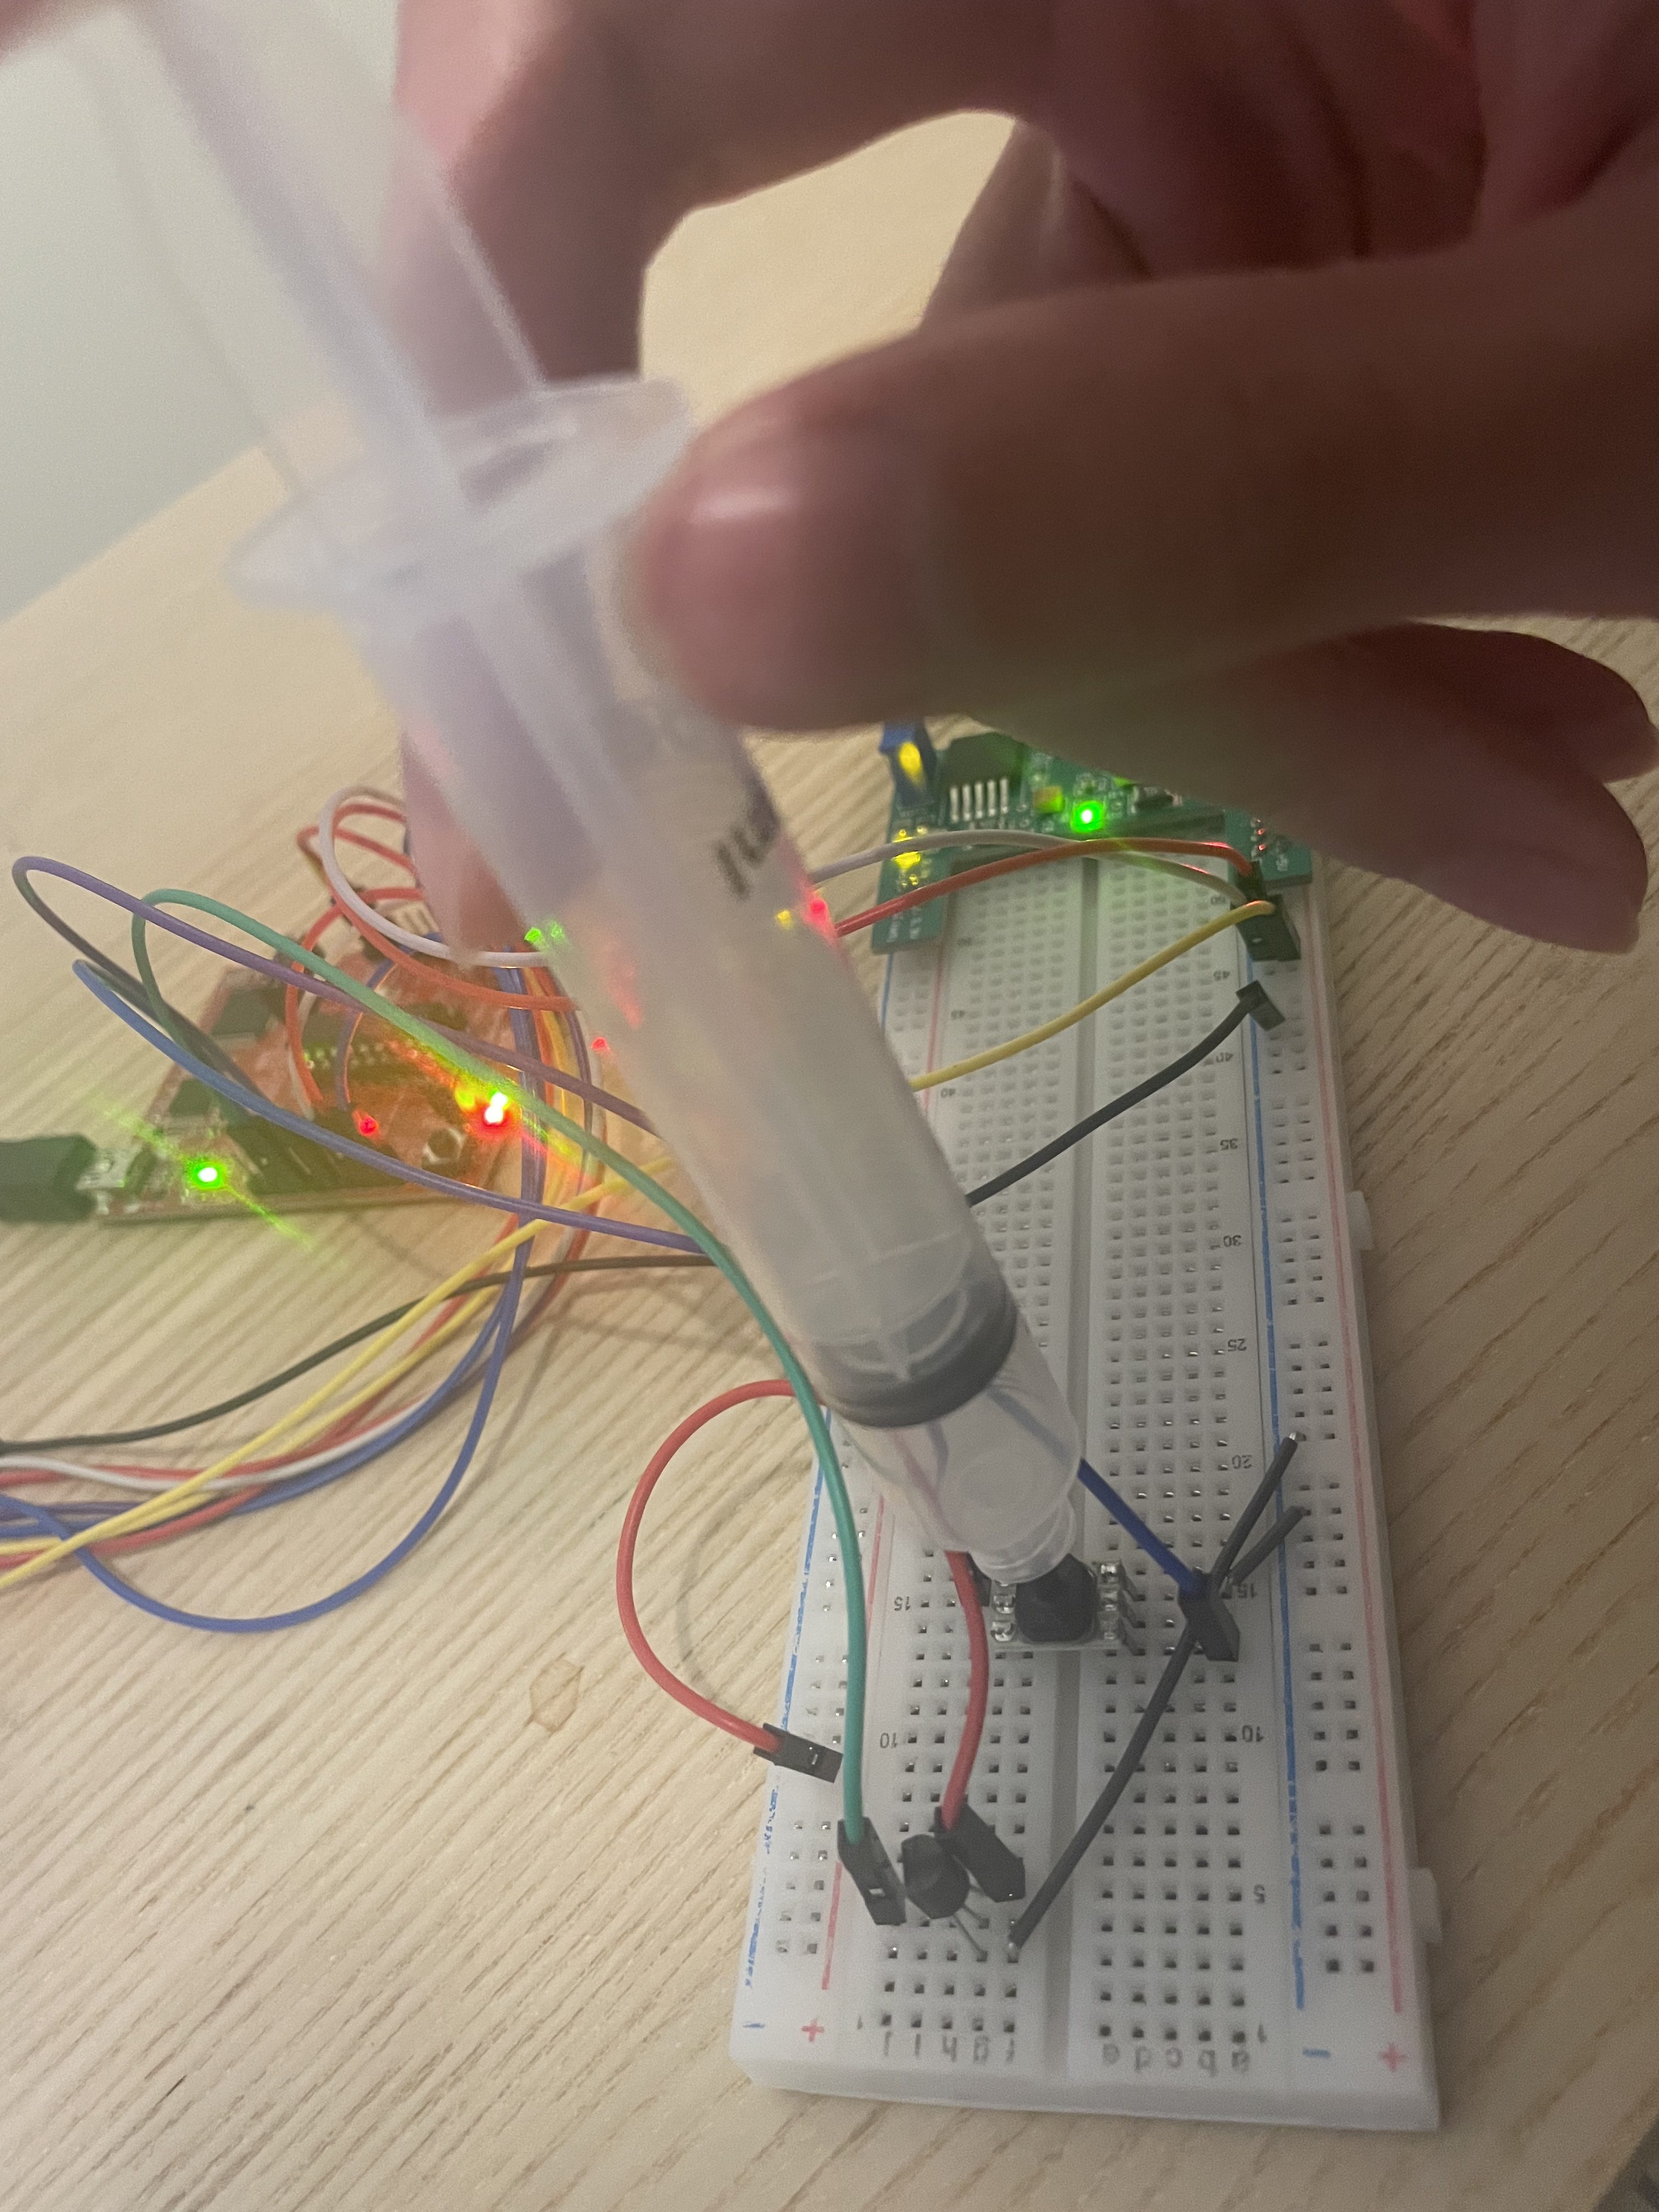
\includegraphics[width=6cm]{Testing Pressure.png}
    \caption{Testing the Pressure Component of the Sensor}
\end{figure} 

\begin{figure}[h]
    \centering
    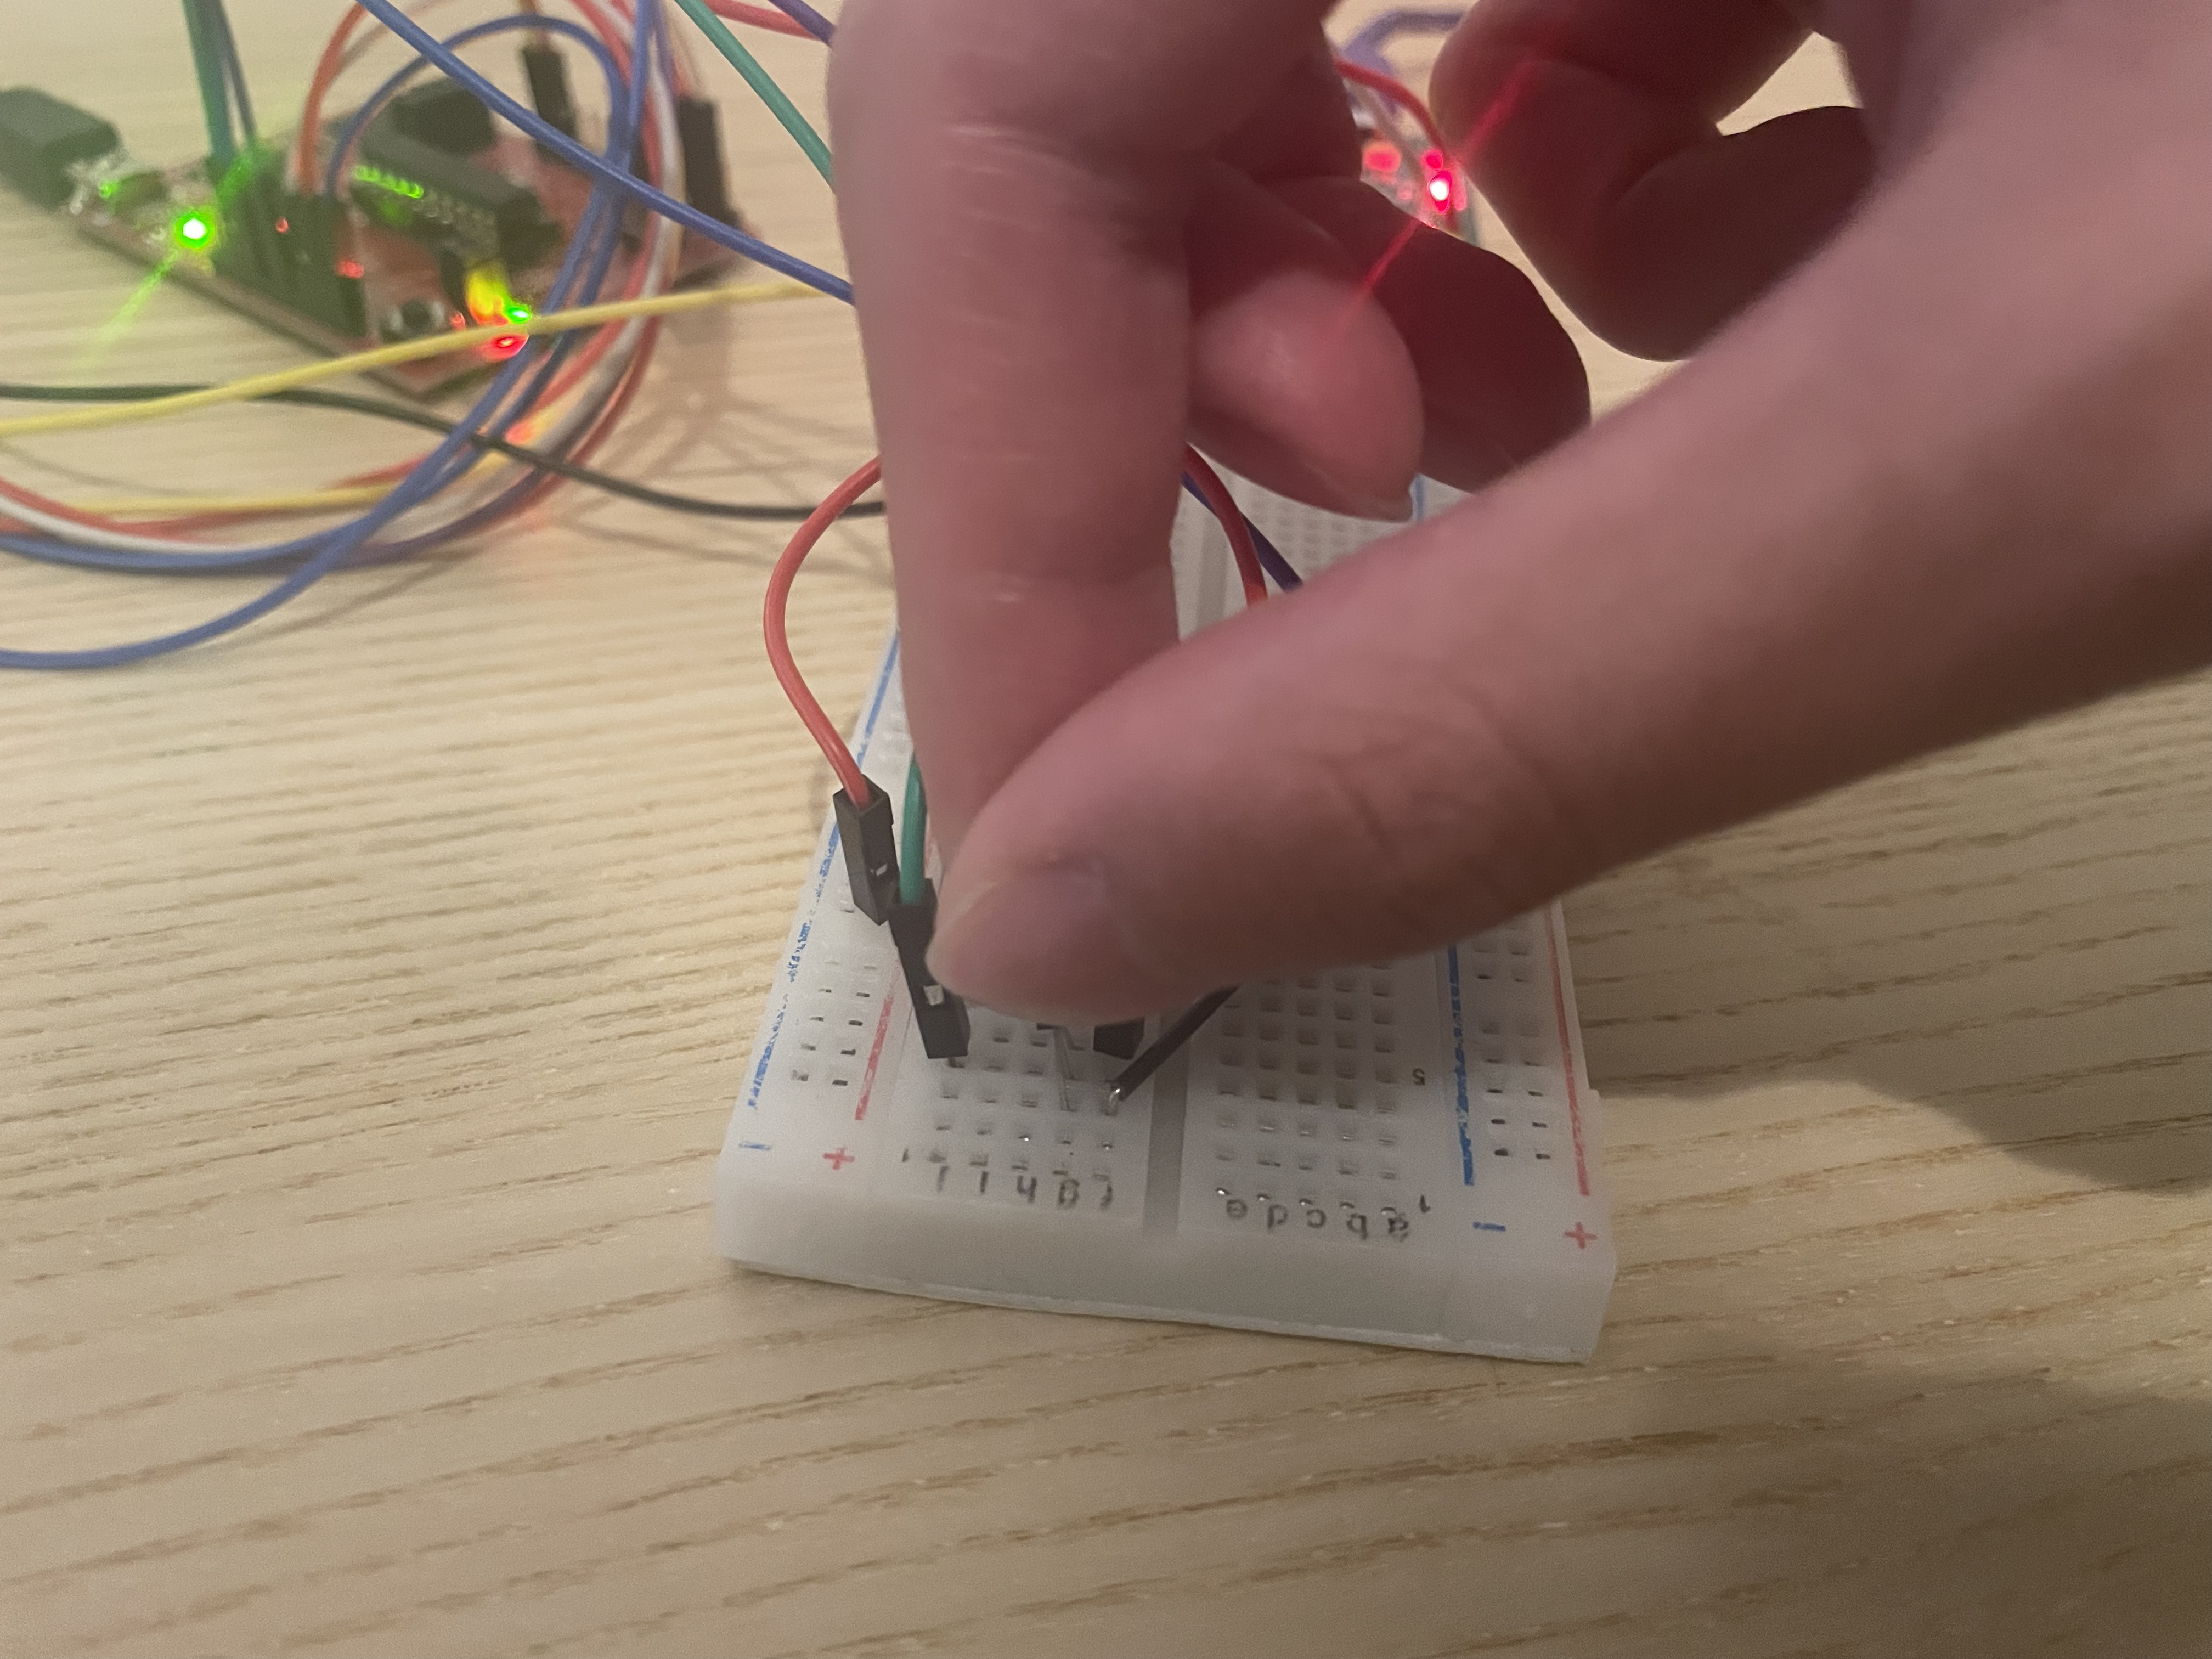
\includegraphics[width=6cm]{Testing Temperature.png}
    \caption{Testing the Temperature Component of the Sensor}
\end{figure} 



\section{Discussions and Improvements}
Overall, the project went smoothly. We faced some difficulties trying to figure out how to obtain more available pins on the microprocessor, and spent a lot of time debugging the code in order to get it work. We also faced some difficulties trying to figure out how to install the temperature and pressure sensor, and nearly burned our sensor due to a wrong installation. But these difficulties were not that's  bad as we had four weeks to get it running smoothly. 

There are definitely several improvements that can be made to this sensor, including allowing the display to display decimal values, which only requires updating the code and will greatly enhance with precision of temperature and pressure measurements with the combined sensor.  Another possible improvement is adding the ability to display negative values, which will greatly enhance the range of temperature values (pressure measurement will always be positive since the lower bound of the sensor working is around 650 millibars). Lastly with the extra pins on P1.5, P1.7 and P2.3 (P1.3 is the button, P1.0 and 1.6 are used for the LED lights), we can add more sensor functions, such as a humidity sensor to this combined sensor complex. 


\section{Conclusion} 
Using the ADC communication and interrupt function of the MSP 430 microprocessor, we have successfully constructed and tested a Combined Temperature and Pressure Sensor with Display, which can be utilized in many different scenarios and have the advantage of easy setup and modification. The sensor is very precise, wjth a $\pm 0.1$ \textdegree C error in temperature sensing, and a $\pm$ 0.5 \textdegree C error in displaying the temperarutre, as well as an relative error(to atmospheric) of 1.5$\%$ for the pressure display. 

It was fun to construct the sensor and the sensor is very stable.  Through this project, we learned about the ADC communication, interruption, while and for loops in C and a lot more of minor details about the MSP 430 microprocessor. Thus, it was definitely worth constructing.

\section{References}

\noindent [1] MuchenHe - Overview. (2022). GitHub. https://github.com/MuchenHe

\noindent [2] TMP36 Temperature Sensor. (n.d.). Adafruit Learning System. 

\noindent https://learn.adafruit.com/tmp36-temperature-sensor

\noindent [3]Honeywell - ABPDANT005PGAA5 - allied ELEC. (n.d.). Retrieved April 11, 2022, from

\noindent https://www.alliedelec.com/product/honeywell/abpdant005pgaa5/70666249/ 

\noindent [4]ADSteele916 - Overview. (2022). GitHub. https://github.com/ADSteele916

\section{Acknowledgements} 
This project was completed at UBC under the supervision of Dr. Andrzej Kotlicki. Special thanks to Dr. Kotliki and the team for helping me complete this project!. Also a big thank you for Alex for allowing me to use his code library. 

\end{document}
